\section{Evaluation}
\label{sec:evaluation}

In this section we analyse the impact of the optimizations from
Section~\ref{sec:op_strategies} on both CPU and GPU implementations.

Our test system is a quad-core Intel Core i7-920 running at 2.67 GHz with
Hyper-threading enabled. For compiling the sequential CPU version we use
\textit{gcc 4.6} with flags ``-O3 -march=native -funroll-loops
-fargument-noalias''. The GPU card is GeForce GTX 480 from Nvidia (Fermi
architecture) with 1.5 GB of total memory and 15 multiprocessors, each with 32
lanes operating at a clock speed of 1.4 GHz. For programming the GPU, we started
from the CPU code base and implemented the algorithms and optimizations with the
established CUDA framework. The device supports CUDA Capability 2.0 which, among
other features, includes the possibility for the same on-chip memory to be used
for both L1 cache and shared memory. It can be configured as either 48 KB of L1
cache and 16 KB of shared memory, or vice versa. We use the first option for the
\textit{evaluation} algorithm in order to cache the accesses to local and global
memories and the temporary register spills. Compilation is done by \textit{Cuda
Toolkit 4.1} with flags ``-arch=sm\_20''.

\begin{figure}[t]
  \begin{subfigure}[t]{1\linewidth}
    \centering
    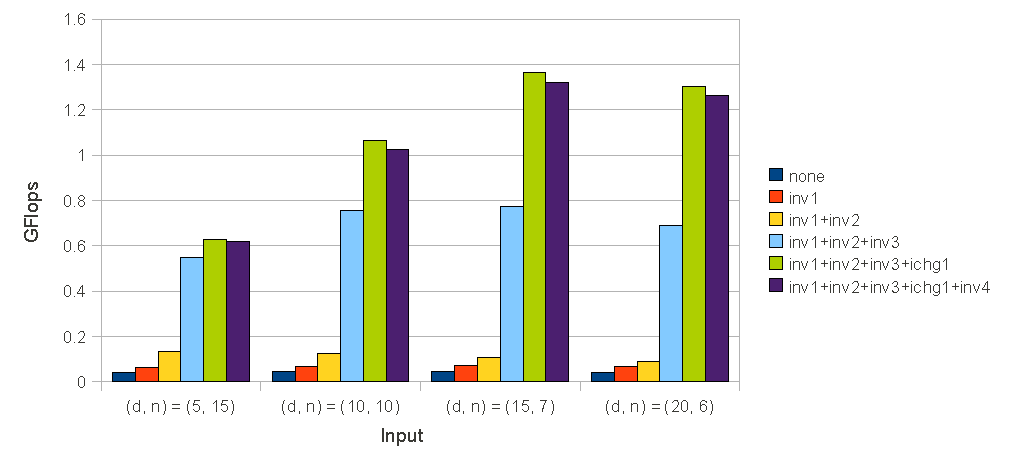
\includegraphics[width=1\linewidth]{hier_cpu} \\
    \caption{CPU}
  \end{subfigure}
  \\ \\
  \begin{subfigure}[t]{1\linewidth}
    \centering
    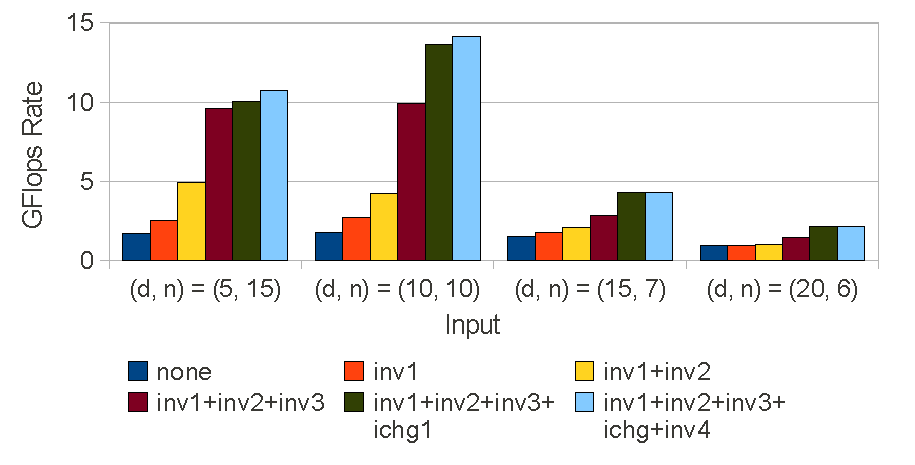
\includegraphics[width=1\linewidth]{hier_gpu}
    \caption{GPU}
  \end{subfigure}
  \caption{Impact of optimizations on the \textit{hierarchization} algorithm.}
  \label{fig:hier_results}
\end{figure}

\begin{figure}[t]
  \begin{subfigure}[t]{1\linewidth}
    \centering
    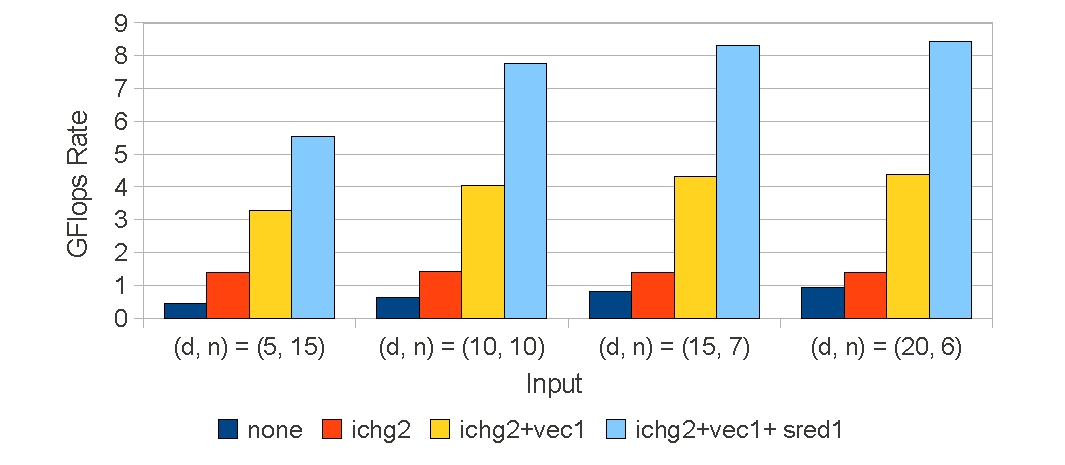
\includegraphics[width=1\linewidth]{eval_cpu} \\
    \caption{CPU}
  \end{subfigure}
  \\ \\
  \begin{subfigure}[t]{1\linewidth}
    \centering
    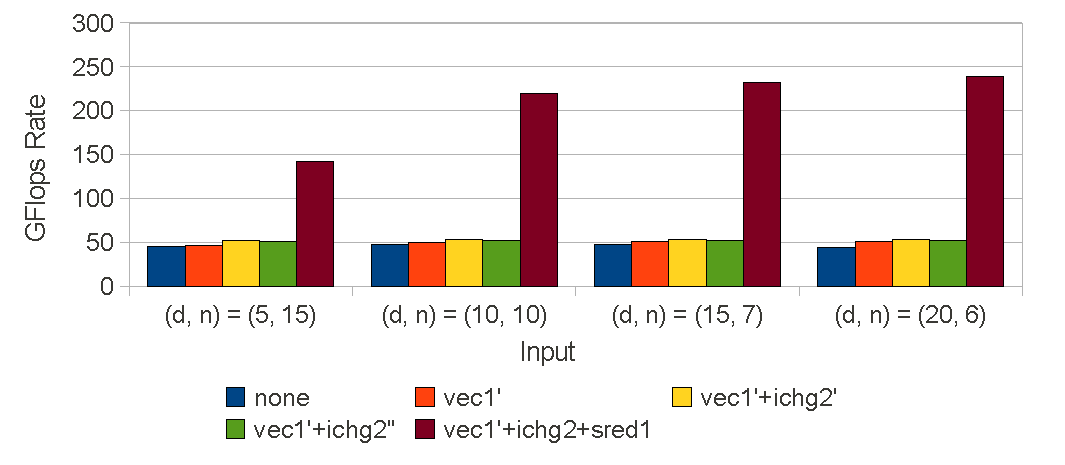
\includegraphics[width=1\linewidth]{eval_gpu}
    \caption{GPU}
  \end{subfigure}
  \caption{Impact of optimizations on \textit{evaluation} algorithm.}
  \label{fig:eval_results}
\end{figure}

We present the impact of our optimizations by measuring the GFlops
rate\footnote{GFlops rate for the GPU version also includes the transfer time
between GPU and main memories.} and comparing with the reference baseline case
where no optimizations are applied. We start with the results obtained for the
\textit{hierarchization} algorithm, depicted in Fig.~\ref{fig:hier_results}. The
tests are done using different configurations, as displayed on the X-axis, where
$d$ is the number of dimensions and $n$ is the number of refinement levels. When
applying all optimizations, a speedup of up to 31x is obtained for CPU and up to
8x for GPU. With the increase in the number of dimensions and the decrease of
the sparse grid size, the speedup for GPU tends to decrease. The explanation is
that the effects of most our optimizations, e.g. improving caching and memory
access patterns, are visible when a high degree of parallelism is achieved, as
is the case for large grids. It is also interesting to notice that \textit{inv4}
brings a drop of performance when applied on top of the other optimizations for
CPU, although for GPU it brings a speedup. This means that if the grids are
small, then it is better to actually do the computations instead of doing memory
lookups, which may result in cache misses. Giving this empirical optimization, a
heterogeneous system could activate or deactivate it at runtime based on the
architecture and compiler used. Lastly, we show that a speedup of 17x is
obtained for the most performant GPU version compared to the corresponding
CPU-based one and a speedup of 6.2x compared to the state-of-the-art GPU
version~\cite{Murarasu:2011:CDS:1941553.1941559}.

In the \textit{evaluation} algorithm, we use $10^{4}$ for CPU and $10^{6}$
for GPU random points, uniformly distributed in the function domain. We
choose a higher number for GPU because the optimizations are visible when
processing a large amount of data. Here we make two empirical observations.
First, since the GFlops rate for CPU remains constant when increasing the number
of interpolation points, both CPU and GPU versions use comparable input data.
Second, we use 8 chunk sizes, i.e. number of interpolation points, for each
warp: 32, 64, 96, 128, 160, 192, 224, and 256, but only choose the best in each
case when comparing the optimizations. For reference, Fig.~\ref{fig:autotune}
shows how increasing this workload influences the results when applying all
optimizations in different input configurations. Although the pattern suggests
an improvement with the increase of thread workload, the results are not
conclusive, which motivates for a careful tuning of the algorithm before
running.

\begin{figure}[t]
  \begin{subfigure}[b]{1\linewidth}
    \centering
    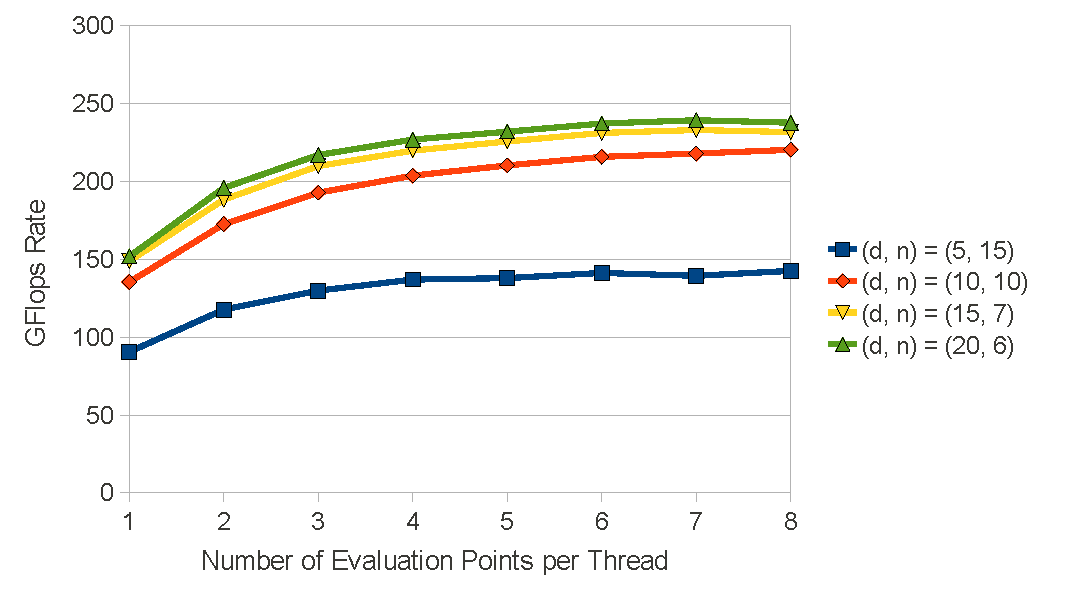
\includegraphics[width=1\linewidth]{autotune}
  \end{subfigure}
  \caption{Varying computational workload for \textit{evaluation}.}
  \label{fig:autotune}
\end{figure}


The results of our tests are presented in Fig.~\ref{fig:eval_results}. Compared
to the CPU versions, the optimizations for GPU are not that effective. The main
reason for this is that, giving the high memory requirement for storing the
interpolation points, we use the GPU global memory. Although caching is
performed, we believe that a higher throughput could be obtained if we could
have stored the results in shared memory. The optimization which brings a clear
speedup is \textit{sred1}, showing that division instructions are still very
expensive on GPUs, fact also emphasized by \cite{cuda}. The GPU version is 28.3x
faster than the CPU one which confirms that sparse grids interpolation technique
is cache friendly and easily parallelizable using our data structure. Compared
to the state-of-the-art GPU version~\cite{Murarasu:2011:CDS:1941553.1941559}, a
speedup of 1.5x is obtained for this algorithm.
